\documentclass[tikz, border=10pt]{standalone}
\usepackage{cmbright}
\usepackage{xcolor}

% Using the accent color from your course document
\definecolor{accent}{HTML}{244470}

\begin{document}

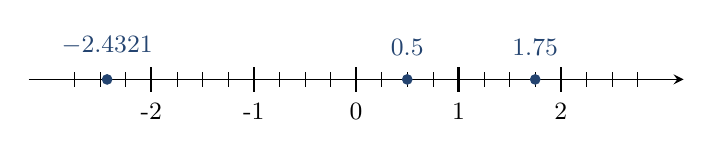
\begin{tikzpicture}[scale=1.3, thick]

    % 1. Main number line (made slightly thicker)
    \draw[->, >=stealth, semithick] (-3.2,0) -- (3.2,0);

    % 2. Minor ticks (every 0.25, excluding integers)
    % We use 'very thin' so they recede into the background
    \foreach \x in {-2.75,-2.5,-2.25,-1.75,-1.5,-1.25,-0.75,-0.5,-0.25,0.25,0.5,0.75,1.25,1.5,1.75,2.25,2.5,2.75} {
        \draw[very thin] (\x,0.07) -- (\x,-0.07);
    }

    % 3. Integer ticks and labels (made 'thick' to stand out)
    \foreach \x in {-2,-1,0,1,2} {
        \draw[thick] (\x,0.12) -- (\x,-0.12);
        \node[below=5pt, font=\small] at (\x,0) {\x};
    }

    % 4. Define a consistent style for the decimal points
    \tikzset{
        pt/.style={circle, fill=accent, inner sep=0pt, minimum size=3pt, draw=accent, thick},
        lbl/.style={above=5pt, font=\small\bfseries, text=accent}
    }

    % Plot the specific points
    \node[pt] at (-2.4321,0) {};
    \node[lbl] at (-2.4321,0) {\(-2.4321\)};

    \node[pt] at (0.5,0) {};
    \node[lbl] at (0.5,0) {\(0.5\)};

    \node[pt] at (1.75,0) {};
    \node[lbl] at (1.75,0) {\(1.75\)};

\end{tikzpicture}

\end{document}